\documentclass[11pt]{article}
\usepackage{url}
\usepackage{pgfplots} 
\pgfplotsset{compat=newest} 
\setlength\topmargin{-0.6cm}   
\setlength\textheight{23.4cm}
\setlength\textwidth{17.0cm}
\setlength\oddsidemargin{0cm} 
\begin{document}
\title{Ling 572 HW2 }
\author{Daniel Campos  \tt {dacampos@uw.edu}}
\date{01/23/2019}
\maketitle 
\section{  Q1 Mallet DT Learner}
\begin{description}
\item [(a)] The command lines:\\ 
mallet import-file --input train.vectors.txt --output train.vectors\\
mallet import-file --input test.vectors.txt --output test.vectors --use-pipe-from train.vectors \\
vectors2classify --training-file train.vectors --testing-file test.vectors --trainer DecisionTree --report test:raw test:accuracy test:confusion train:confusion train:accuracy \textgreater de1.stdout 2 \textgreater de1.stderr \\
tail de1.stdout 
\item [(b)] What are the training accuracy and the test accuracy? \\
Train:0.1781 \\
Test: 0.1
\end{description}
\section{ Q2 Mallet Different depth}
\begin{table}[h]
\centering
\caption{Mallet's DT learner with different depths}
See table 1. \\ B) Looking at table 1 we can see that as we train deeper or model learns the distribution of the train set much better but that doesnt necissarily mean that it will perform better on our test set. This, as is common with most ML shows that we must be careful when focusing on performance on the train set because it may mean nothing in terms of true model performance.
\label{table1}
\begin{tabular}{|l|l|l|} \hline
Depth   & Training accuracy & Test accuracy \\ \hline
1       & 0.1393 & 0.1033  \\ \hline
2       & 0.1419 & 0.12 \\ \hline
4       &  0.1781 & 0.10 \\ \hline
10      & 0.6285   & 0.1133 \\ \hline
20      &  0.9970 & 0.1367 \\ \hline
50      &  1  & 0.1367 \\ \hline
\end{tabular}
\end{table}
\section{ Q3 build\_dt.sh} 
See table 2 and table 3
\begin{table}[hbtp]
\centering
\caption{build\_dt.sh min\_gain=0}
\label{table2}
\begin{tabular}{|l|l|l|l|} \hline
Depth   & Training accuracy & Test accuracy & CPU time (in minutes)\\ \hline
1       & 0.4530 & 0.4167 & 1  \\ \hline
2       &  0.5207 & 0.53  & 2  \\ \hline
4       & 0.6377 & 0.5267  & 3  \\ \hline
10      &0.7511 & 0.5933  & 10 \\ \hline
20      & 0.8541 & 0.6733  & 11  \\ \hline
50      & 0.96333  & 0.6933 &   33    \\ \hline
\end{tabular}
\end{table}
\begin{table}[hbtp]
\centering
\caption{build\_dt.sh min\_gain=0.1}
\label{table3}
\begin{tabular}{|l|l|l|l|} \hline
Depth   & Training accuracy & Test accuracy & CPU time (in minutes)\\ \hline
1       & 0.6014& 0.54 &3  \\ \hline
2       & 0.52  & 0.53  & 2  \\ \hline
4       & 0.6014 &0.54 &4  \\ \hline
10      & 0.6014 &0.54& 3  \\ \hline
20      &  0.6014 &0.54& 3 \\ \hline
50      & 0.6014 & 0.54  &  2    \\ \hline
\end{tabular}
\end{table}
\section{ Q4}
\begin{tikzpicture} 
\begin{axis}[
  axis x line=center,
  axis y line=center,
  xtick={-20,-10,...,30},
  ytick={-10,0,...,30},
  xlabel={$x$},
  ylabel={$y$},
  xlabel style={below right},
  ylabel style={above left},
  xmin=-22,
  xmax=32,
  ymin=-12,
  ymax=32]
\draw[red, dashed, very thick]  (20,10) rectangle (30,30) node {L1};
\draw[blue, dashed, very thick]  (10,10) rectangle (20,30) node {L2};
\draw[green, dashed, very thick] (0,-10) rectangle (10,30) node {L3};
\draw[orange, dashed, very thick](0,-10) rectangle (10,30) node {L4};
\draw[pink, dashed, very thick] (-20,20) rectangle (0,30) node {L5};
\draw[yellow, dashed, very thick] (-20,-10) rectangle (0,20) node {L6};
\draw(-20,-10) rectangle (-10,20) node {L7};
\end{axis}
\end{tikzpicture}
\section{Q5: Notes}
I believe everything is working great except when the depth of the tree is high the run time is slow. It me a while to move from pandas data frames to numpy arrays and when I did so my programs started going much faster. This assignment really showcases how improtant some of the hyperparameters like max dcepth and min gain are to both affect the runtime and the  accuracy. 
\end{document}



